\documentclass[dvipdfmx,11pt]{beamer}

%全体設定
%\AtBeginDvi{\special{pdf:tounicode 90ms-RKSJ-UCS2}}

\usepackage{bxdpx-beamer}% dvipdfmxなので必要
\usepackage{pxjahyper}
\usepackage{minijs}
\usepackage{otf}
\usepackage{amssymb,amsmath}
\usepackage{hyperref}
\usepackage[absolute,overlay]{textpos}
\usepackage{comment}
\usepackage{colortbl}
\usepackage{graphicx}
\usepackage{tikz}
\usetikzlibrary{positioning}
\usetikzlibrary{shadows}
\usepackage{listings}
\usepackage{plistings}
\def\lstlistingname{コード}

\renewcommand{\kanjifamilydefault}{\gtdefault}
%%\usetheme{Frankfurt}
\usetheme{Warsaw}
\setbeamertemplate{navigation symbols}{} %スライドのボタン?(右下のやつ)を消す
\setbeamersize{text margin left=1.5em,text margin right=1.5em} % 余白なくすやつ

\title{解集合プログラミングを用いた\\配電網問題の解法に関する考察}
\author{山田 健太郎}
\date{卒業研究発表会\\2020年2月20日}
\institute{番原研究室}

%% テンプレ 
\begin{comment}

%%%%%%%%%%%%%%%%%%%%%%%%%%%%%%%%%%%%%%%%%%%%%%%%%%
%% タイトル
%%%%%%%%%%%%%%%%%%%%%%%%%%%%%%%%%%%%%%%%%%%%%%%%%%
\begin{frame}\frametitle{}
\end{frame}

\end{comment}

%###########################################################
%# 本文 ####################################################
%###########################################################
\begin{document}

%%%%%%%%%%%%%%%%%%%%%%%%%%%%%%%%%%%%%%%%%%%%%%%%%%
%% タイトル 
%%%%%%%%%%%%%%%%%%%%%%%%%%%%%%%%%%%%%%%%%%%%%%%%%%
\begin{frame}\frametitle{}
  \titlepage
\end{frame}

%%%%%%%%%%%%%%%%%%%%%%%%%%%%%%%%%%%%%%%%%%%%%%%%%%
% 配電網
%%%%%%%%%%%%%%%%%%%%%%%%%%%%%%%%%%%%%%%%%%%%%%%%%%
\begin{frame}\frametitle{配電網問題}
 \begin{alertblock}{}
  \centering
  求解困難な組合せ最適化問題の一種
 \end{alertblock}

 \begin{itemize}
  \item  \alert{配電網}とは,変電所と,家庭や工場などから構成される
		 電力供給経路のネットワークである.
  \item  配電網の構成技術はスマートグリッドや,災害時の障害箇所の迂回構成などを支える
		 重要な基盤技術として期待されている.
  \item  \alert{配電網問題}とは,
		 \begin{itemize}
		  \item \structure{トポロジ制約}と\structure{電気制約}から構成.
		  \item 損失電力を最小にするスイッチの開閉状態を求めることが目的.
		 \end{itemize}
  \item フロンティア法を用いた解法が提案されている[井上ほか '12]. 
		\begin{itemize}
		 \item ERATO湊離散構造処理系プロジェクトの成果.
		 \item 実用規模の配電網問題(\structure{\textbf{スイッチ数468個}})の最適解を発見.
		\end{itemize}
 \end{itemize}

 \vspace{-0.25cm}
 \pause
 \begin{alertblock}{}
  トポロジ制約のみの配電網問題は,グラフと根と呼ばれる特別なノードから,
  \alert{根付き全域森}を求める部分グラフ探索問題に帰着できる.
 \end{alertblock}
  
\end{frame}

%%%%%%%%%%%%%%%%%%%%%%%%%%%%%%%%%%%%%%%%%%%%%%%%%%
%% 根付き全域森
%%%%%%%%%%%%%%%%%%%%%%%%%%%%%%%%%%%%%%%%%%%%%%%%%%
\begin{frame}\frametitle{根付き全域森(Spanning Rooted Forest)}

 \begin{block}{根付き全域森~~[川原$\cdot$湊 '12]}
  グラフ$G=(V,E)$と,
  \alert{根}と呼ばれる$V$上のノードが与えられたとき,
  $G$上の根付き全域森とは,以下の条件を満たす$G$の部分グラフ$G'=(V,E'),\ E' \subseteq E$である.
  \begin{enumerate}
   \item $G'$はサイクルを持たない. (\alert{非閉路制約})
   \item $G'$の各連結成分は,ちょうど1つの根を含む. (\alert{根付き連結制約})
  \end{enumerate}
 \end{block}

 \begin{exampleblock}{根付き全域森の例}
  \begin{columns}
   \begin{column}{0.45\textwidth}
	\centering
	%%%%%%%%%%%%%%%%%%%%%%%%%%%%%%%%%%%%%%%%%%%%%%%%%%
% 根付き全域森の例
%%%%%%%%%%%%%%%%%%%%%%%%%%%%%%%%%%%%%%%%%%%%%%%%%%

\begin{tikzpicture}[scale=0.5]

 % 設定
 \tikzset{node/.style={circle,draw=black,fill=white}}

 \definecolor{edge1}{RGB}{191,0,0}
 \definecolor{node1}{RGB}{249,200,200}
 \definecolor{edge3}{RGB}{38,38,134}
 \definecolor{node3}{RGB}{200,200,249}

 % 補助線
 % \draw [help lines,blue] (0,0) grid (20,6);

 % 入力されるグラフ
 % node %
 \node[circle, ultra thick,draw=edge1,fill=node1] (in1) {1};
 \node[node,right= of in1] (in2){2};
 \node[circle, ultra thick, draw=edge3,fill=node3, right=of in2](in3){3};
 \node[node,below= of in1] (in4){4};
 \node[node,below= of in2] (in5){5};
 \node[node,below= of in3] (in6){6};

 % 辺
 \foreach \u / \v in {in1/in2,in2/in3,in1/in4,in2/in5,in3/in6,in4/in5,in5/in6}
 \draw (\u) -- (\v);

\end{tikzpicture}

%%%%%%%%%%%%%%%%%%%%%%%%%%%%%%%%%%%%%%%%%%%%%%%%%%%%%%%%%%
%%% Local Variables:
%%% mode: japanese-latex
%%% TeX-master: ``slide''
%%% End:

   \end{column}
   \begin{column}{0.45\textwidth}
	\centering
	%%%%%%%%%%%%%%%%%%%%%%%%%%%%%%%%%%%%%%%%%%%%%%%%%%
% 根付き全域森の例
%%%%%%%%%%%%%%%%%%%%%%%%%%%%%%%%%%%%%%%%%%%%%%%%%%

\begin{tikzpicture}[scale=0.5]

 % 設定
 \tikzset{node/.style={circle,draw=black,fill=white}}

 \definecolor{edge1}{RGB}{191,0,0}
 \definecolor{node1}{RGB}{249,200,200}
 \definecolor{edge3}{RGB}{38,38,134}
 \definecolor{node3}{RGB}{200,200,249}

 % 補助線
 % \draw [help lines,blue] (0,0) grid (20,6);

 % node %
 \node[circle, ultra thick, draw=edge1, fill=node1](out1){1};
 \node[node, fill=node1, right=of out1] (out2){2};
 \node[circle, ultra thick, draw=edge3,fill=node3, right=of out2](out3){3};
 \node[node, fill=node1, below=of out1] (out4){4};
 \node[node, fill=node3, below=of out2] (out5){5};
 \node[node, fill=node3, below=of out3] (out6){6};

 \foreach \u / \v in {out1/out2,out1/out4}
 \draw [very thick, edge1] (\u) -- (\v);

 \foreach \u / \v in {out3/out6,out5/out6}
 \draw [very thick, edge3](\u) -- (\v);

\end{tikzpicture}

%%%%%%%%%%%%%%%%%%%%%%%%%%%%%%%%%%%%%%%%%%%%%%%%%%%%%%%%%%
%%% Local Variables:
%%% mode: japanese-latex
%%% TeX-master: ``slide''
%%% End:

   \end{column}
  \end{columns}


 \end{exampleblock}
 
\end{frame}

%%%%%%%%%%%%%%%%%%%%%%%%%%%%%%%%%%%%%%%%%%%%%%%%%%
%% ASP
%%%%%%%%%%%%%%%%%%%%%%%%%%%%%%%%%%%%%%%%%%%%%%%%%%
\begin{frame}\frametitle{解集合プログラミング(Answer Set Programming; ASP)}
 \begin{itemize}
  \item \structure{ASP言語}は一階論理に基づく知識表現言語の一種である.
  \item \structure{ASPシステム}は論理プログラムから安定モデル意味論[Gelfond and Lifschitz '88]に
		基づく解集合を計算するシステムである.
  \item 近年ではSAT技術を応用した高速ASPシステムが実現され,システム検証,プランニング,
		システム生物学など様々な分野への応用が拡大している.
 \end{itemize}

 \begin{alertblock}{ASP技術を組合せ最適化問題に用いる利点}
   \begin{itemize}
	\item ASP言語の高い表現力を活かし,記号的な制約を簡潔に記述可能.
	\item ASPMT技術を用いて,様々な背景理論ソルバーと連携可能.
	\item 充足不能コアを用いた効率的な最適値探索が利用可能.
%	\item ASPシステムの持つ高い拡張性により,新たな制約の追加が容易.
   \end{itemize}
 \end{alertblock}

\end{frame}

%%%%%%%%%%%%%%%%%%%%%%%%%%%%%%%%%%%%%%%%%%%%%%%%%%
%% 研究目的
%%%%%%%%%%%%%%%%%%%%%%%%%%%%%%%%%%%%%%%%%%%%%%%%%%
\begin{frame}\frametitle{研究目的}
 \begin{alertblock}{目的}
  % \centering
  ASP技術を活用して,大規模な配電網問題を効率良く解くシステムの\\構築を目指す.
 \end{alertblock}

 \begin{block}{研究内容}
  \begin{enumerate}
   \item \structure{根付き全域森問題を解く,2種類のASP符号化を考案した.}
   % \begin{itemize}
   % 	\item 上限,下限に基づく符号化.
   % 	\item ASP言語の表現性を利用した符号化.
	 % \end{itemize}
   \item \structure{実用規模の問題,及び,より大規模な問題を用いた評価実験.}
   % \begin{itemize}
   % 	\item 問題の規模に関する比較評価.
   % 	\item 生成される制約の数の比較評価.
   % \end{itemize
   \item 遷移問題へ拡張し,その符号化を考案した.
   \begin{itemize}
	\item ある配電網の構成(初期状態)から,目的とする配電網の構成(目的状態)を得るための,
		  スイッチの切替手順を求める問題.
   \end{itemize}
  \end{enumerate}
  
 \end{block}
 
\end{frame}

\begin{frame}\frametitle{ASPを用いた根付き全域森問題の解法}
 
 \begin{figure}[htbp]
  \centering
  %%%%%%%%%%%%%%%%%%%%%%%%%%%%%%%%%%%%%%%%%%%%%%%%%%
%% ASPで配電網問題を解く流れの図
%%%%%%%%%%%%%%%%%%%%%%%%%%%%%%%%%%%%%%%%%%%%%%%%%%
\begin{tikzpicture}

 \definecolor{edge}{RGB}{38,38,134}
 \definecolor{node}{RGB}{220,220,249}

 \definecolor{alert_edge}{RGB}{191,0,0}
 \definecolor{alert_node}{RGB}{249,200,200}

 \definecolor{example_edge}{RGB}{0,96,0}
 \definecolor{example_node}{RGB}{230,239,230}

 \tikzset{block/.style={rectangle, very thick, draw=edge, fill=node, text centered, 
 rounded corners, text width=3cm, minimum height=1.5cm,minimum width=3cm}};

 \tikzset{alertblock/.style={rectangle, very thick, draw=alert_edge, fill=alert_node, 
 text centered, rounded corners, text width=3cm, minimum height=1.5cm, minimum width=3cm}};

\tikzset{exampleblock/.style={rectangle, very thick, draw=example_edge, fill=example_node, text centered, 
 rounded corners, text width=3cm, minimum height=1cm,minimum width=1cm}};


 \node[block](fact){問題インスタンス\\(ASPファクト)};
 \node[exampleblock, below right=0.2cm and 1.5cm of fact] (pre){変換\\(配電網$\rightarrow$ SRF)};
 \node[alertblock, below=3cm of fact] (srf){根付き全域森\\問題(SRF)};
 \node[exampleblock, above right=0.3cm and 1.5cm of srf](decode){復元\\(SRF $\rightarrow$配電網)};
 \node[alertblock, below right=0.3cm and 1.5cm of decode](cur){電気制約};
 \node[block, above right=0.3cm and 1.5cm of pre] (ans){問題の解};
 \node[below=0.65cm of fact] (point1){};
 \node[right=3cm of srf] (point2){};

 \draw[very thick, ->] (fact)--(srf);
 \draw[very thick, ->] (srf)--(cur);
 \draw[very thick, ->] (cur)--(ans);
 \draw[very thick, ->] (pre)--(point1);
 \draw[very thick, ->] (decode)--(point2);

\end{tikzpicture}
 \end{figure}

 \vspace{-0.5cm}
 \begin{exampleblock}{}
  \begin{enumerate}
   \item 与えられた問題インスタンスをASPのファクト形式に変換する.
   \item 変換した問題と,根付き全域森問題を解くASP符号化を結合し,
		 ASPシステムを用いて解を求める.
  \end{enumerate}
 \end{exampleblock}
\end{frame}

%%%%%%%%%%%%%%%%%%%%%%%%%%%%%%%%%%%%%%%%%%%%%%%%%%
%% 提案手法
%%%%%%%%%%%%%%%%%%%%%%%%%%%%%%%%%%%%%%%%%%%%%%%%%%
\begin{frame}\frametitle{提案するASP符号化}
 
\begin{itemize}
 \item  根付き全域森問題に対する,2種類のASP符号化を考案した.
 \item $|V|$はグラフのノード数,$|R|$は根ノード数をそれぞれ表す.
\end{itemize}
 
\begin{table}[t]
 \centering
 %%%%%%%%%%%%%%%%%%%%%%%%%%%%%%%%%%%%%%%%%%%%%%%%%%%%%%%%%%%%%%%%
\chapter{ハミルトン閉路問題および関連問題のASP符号化}\label{chap:proposal}
%%%%%%%%%%%%%%%%%%%%%%%%%%%%%%%%%%%%%%%%%%%%%%%%%%%%%%%%%%%%%%%% 

%%%%
\begin{figure}[h]
  \centering
  \thicklines
  \setlength{\unitlength}{1.2pt}
  \small\footnotesize\scriptsize
  \begin{picture}(280,57)(4,-10)
    \put(  0, 20){\dashbox(50,24){\shortstack{HCP問題\\インスタンス}}}
    \put( 60, 20){\framebox(50,24){変換器}}
    \put(120, 20){\dashbox(50,24){\shortstack{ASPファクト}}}
    \put(120,-10){\dashbox(50,24){\shortstack{ASP符号化\\(論理プログラム)}}}
    \put(180, 20){\framebox(50,24){ASPシステム}}
    \put(240, 20){\dashbox(50,24){\shortstack{HCP問題\\の解}}}
    \put( 50, 32){\vector(1,0){10}}
    \put(110, 32){\vector(1,0){10}}
    \put(170, 32){\vector(1,0){10}}
    \put(230, 32){\vector(1,0){10}}
    \put(170, +2){\line(1,0){4}}
    \put(174, +2){\line(0,1){30}}
  \end{picture}  
\caption{ASP を用いたハミルトン閉路問題(HCP)の解法}
\label{fig:arch}
\end{figure}
%%%%

%\begin{figure}[tbp]
\tikz{
  %1ノード目
  \path[draw=black, fill=blue!20, rounded corners=5pt]%線の設定
  node[at={(0.75,0.75)}] {問題}%文字を入れる
  (0,0) --(1.5,0) --(1.5,1.5) --(0,1.5) --cycle;%外周
  %2ノード目
  \path[draw=black, fill=blue!20, rounded corners=5pt, shift={(3,0)}]
  node[at={(0.75,0.75)}] {
    \begin{tabular}{c}
      ASP\\
      ファクト
    \end{tabular}
  }
  (0,0) --(1.5,0) --(1.5,1.5) --(0,1.5) --cycle;
  %3ノード目文字が複数行
  \path[draw=black, fill=green!20, rounded corners=5pt, shift={(6,0)}]
  node[at={(0.75,0.75)}] {
    \begin{tabular}{c}
      ASP\\
      システム
    \end{tabular}
  }
  (0,0) --(1.5,0) --(1.5,1.5) --(0,1.5) --cycle;
  %4ノード目文字が複数行
  \path[draw=black, fill=blue!20, rounded corners=5pt, shift={(9,0)}]
  node[at={(0.75,0.75)}] {解集合}
  (0,0) --(1.5,0) --(1.5,1.5) --(0,1.5) --cycle;
  %5ノード目文字が複数行
  \path[draw=black, fill=red!20, rounded corners=5pt, shift={(3,-3)}]
  node[at={(0.75,0.75)}] {
    \begin{tabular}{c}
      ASP\\
      符号化
    \end{tabular}
  }
  (0,0) --(1.5,0) --(1.5,1.5) --(0,1.5) --cycle;
  \draw[arrows=->] (1.5,0.75) --(3.0,0.75);
  \draw[arrows=->,shift={(3,0)}] (1.5,0.75) --(3.0,0.75);
  \draw[arrows=->,shift={(6,0)}] (1.5,0.75) --(3.0,0.75);
  \draw[arrows=->] (4.5,-2.25) --(6.0,0.5);
}
\caption{ASPを用いた解法}
\label{aspmethod}
\end{figure}


ASP を用いたハミルトン閉路問題および関連問題の解法について述べる.
図~\ref{fig:arch}に,解法の流れを示す.
与えられたハミルトン閉路問題は ASP ファクトに変換され,
ハミルトン閉路問題を解く ASP 符号化と結合され,
ASP システムによって解が計算される.
本論文では,ASP システムとして{\clingo}を用いる.

%%%%%%%%%%%%%%%%%%%%%%%%%%%%%%%%%%%%%%%%%%%%%%%%%%%%%%%%%%%%%%%%%%%%%%%
\section{ASPファクト形式}
%%%%%%%%%%%%%%%%%%%%%%%%%%%%%%%%%%%%%%%%%%%%%%%%%%%%%%%%%%%%%%%%%%%%%%%

%%%%%%%%%%%%%%%%%%%%%%%%%%%%%%
\begin{figure}[t]
\begin{center}
\begin{tikzpicture}
  %ノード1  
  \draw(4,2) circle (0.5)
  node[at={(4.1,2.1)}] {
    \begin{tabular}{c}
      1
    \end{tabular}
  };
  %ノード2  
  \draw(4,0) circle (0.5)
  node[at={(4.1,0.1)}] {
    \begin{tabular}{c}
      2
    \end{tabular}
  };
  %ノード3  
  \draw(6,2) circle (0.5)
  node[at={(6.1,2.1)}] {
    \begin{tabular}{c}
      3
    \end{tabular}
  };
  %ノード4  
  \draw(6,0) circle (0.5)
  node[at={(6.1,0.1)}] {
    \begin{tabular}{c}
      4
    \end{tabular}
  };
  %ノード5  
  \draw(8,2) circle (0.5)
  node[at={(8.1,2.1)}] {
    \begin{tabular}{c}
      5
    \end{tabular}
  };
  %ノード6  
  \draw(8,0) circle (0.5)
  node[at={(8.1,0.1)}] {
    \begin{tabular}{c}
      6
    \end{tabular}
  };
\draw(4,0.5) --(4,1.5);
\draw(6,0.5) --(6,1.5);
\draw(8,0.5) --(8,1.5);
\draw(4.5,0) --(5.5,0);
\draw(4.5,2) --(5.5,2);
\draw(6.5,0) --(7.5,0);
\draw(6.5,2) --(7.5,2);
\end{tikzpicture}

\caption{入力となる重み付き無向グラフの例}
\label{graphexample}
\end{center}
\end{figure}
%%%%%%%%%%%%%%%%%%%%%%%%%%%%%%

%%%%%%%%%%%%%%%%%%%%%%%%%%%%%%
\lstinputlisting[float=t,caption={%
図~\ref{graphexample}のASPファクト表現},%
captionpos=b,frame=single,label=code:graph_example.lp,%
numbers=none,%
breaklines=true,%
columns=fullflexible,keepspaces=true,%
basicstyle=\ttfamily\scriptsize]{code/graph_example.lp}
%%%%%%%%%%%%%%%%%%%%%%%%%%%%%%


本節では,最短ハミルトン閉路問題の例にとって,
入力となる重み付き無向グラフ(図~\ref{graphexample})の
ASP ファクト形式について説明する.
%
このグラフは,頂点数が6,辺の数が7であり,辺に付けられた値は距離を表す.
コード~\ref{code:graph_example.lp}に,ASPファクト形式を示す.
%
アトム\code{node/1}は頂点,\code{edge/2}は辺,\code{cost/3}は距離を表す.
例えば,\code{cost(1,2,3)}は,辺\code{edge(1,2)}の距離が3であることを
表している.

%%%%%%%%%%%%%%%%%%%%%%%%%%%%%%%%%%%%%%%%%%%%%%%%%%%%%%%%%%%%%%%%%%%%%%%
\section{ハミルトン閉路問題の ASP 符号化}\label{hamiltonianasp}
%%%%%%%%%%%%%%%%%%%%%%%%%%%%%%%%%%%%%%%%%%%%%%%%%%%%%%%%%%%%%%%%%%%%%%%

ハミルトン閉路問題は,与えられたグラフの全頂点をちょうど一度ずつ通る閉
路(ハミルトン閉路)が存在するかどうかを判定する問題である.
$G=(V,E)$にハミルトン閉路が存在する必要十分条件は,
以下の2つの制約を満たす部分グラフ$G'=(V,E')$が存在することである.

\begin{itemize}
\item $G'$の各頂点の次数が2 (次数制約)
\item $G'$が連結である (連結制約)
\end{itemize}

本論文では,前者を\textbf{次数制約},後者を\textbf{連結制約}と呼ぶ.
ハミルトン路問題は,ハミルトン閉路問題から始点と終点が一致するという閉
路の条件を取り除いたものである.
ハミルトン路問題では,次数制約は以下のように変わる.

\begin{itemize}
\item 始点と終点の次数が1,他の頂点の次数が2
\end{itemize}

以下では,ハミルトン閉路問題に対する3つの ASP 符号化
\textsf{undirected},\textsf{directed},\textsf{acyclicity}
を提案する.

%%%%%%%%%%%%%%%%%%%%%%%%%%%%%%%%%%%%%%%%%%%%%%%%%%%%%%%%%%%%%%%%%%%%%%%
\subsection{\textsf{undirected}符号化}
%%%%%%%%%%%%%%%%%%%%%%%%%%%%%%%%%%%%%%%%%%%%%%%%%%%%%%%%%%%%%%%%%%%%%%%

%%%%%%%%%%%%%%%%%%%%%%%%%%%%%%
\lstinputlisting[float=t,caption={%
\textsf{undirected}符号化},%
captionpos=b,frame=single,label=code:hamilton1.lp,%
numbers=left,%
breaklines=true,%
columns=fullflexible,keepspaces=true,%
basicstyle=\ttfamily\footnotesize]{code/hamilton1.lp}
%%%%%%%%%%%%%%%%%%%%%%%%%%%%%%

\textsf{undirected}符号化は,ハミルトン閉路問題の次数制約と連結制約を,
ASP の一貫性制約で表した基本的な符号化である.
コード~\ref{code:hamilton1.lp}に,\textsf{undirected}符号化を示す.
この符号化は,ハミルトン閉路問題とハミルトン路問題の両方に対応している.
符号化中の\code{s}は始点の頂点番号,\code{t}は終点の頂点番号を表し,こ
れらは実行時に与えられる.
ここでは,ハミルトン閉路問題(\code{s}=\code{t})の場合について説明する.

\begin{itemize}
\item 1行目のルールは,各辺\code{edge(X,Y)}に対して,その辺がハミルト
  ン閉路に含まれるかどうかを意味するアトム\code{in(X,Y)}を選択子を用い
  て導入している.
\item 次数制約は3行目のルールで表される.このルールは,
  各頂点\code{node(X)}に対して,その次数の和が2に等しいことを個数制約
  を使って表している.
\item 連結制約は11行目のルールで表される.
ある頂点\code{X}が始点\code{s}から到達可能であることを意味する補助アト
ム\code{reached(X)}を導入する.
8行目のルールは,始点\code{s}が到達可能あることを表している.
9行目のルールは,各辺\code{X}--\code{Y}に対して,その辺がハミルトン閉
路に含まれ(\code{in(X,Y)}),かつ,頂点\code{X}が始点から到
達可能であれば(\code{reached(X)}),\code{Y}も到達可能であることを表している.
10行目は9行目と同様であるが,辺\code{Y}--\code{X}の場合を表している.
11行目のルールは,各頂点\code{node(X)}が始点から到達可能でなければな
らないことを一貫性制約を使って表している.
\end{itemize}

%%%%%%%%%%%%%%%%%%%%%%%%%%%%%%%%%%%%%%%%%%%%%%%%%%%%%%%%%%%%%%%%%%%%%%%
\subsection{\textsf{directed}符号化}
%%%%%%%%%%%%%%%%%%%%%%%%%%%%%%%%%%%%%%%%%%%%%%%%%%%%%%%%%%%%%%%%%%%%%%%

%%%%%%%%%%%%%%%%%%%%%%%%%%%%%%
\lstinputlisting[float=t,caption={%
\textsf{directed}符号化},%
captionpos=b,frame=single,label=code:hamilton2.lp,%
numbers=left,%
breaklines=true,%
columns=fullflexible,keepspaces=true,%
basicstyle=\ttfamily\footnotesize]{code/hamilton2.lp}
%%%%%%%%%%%%%%%%%%%%%%%%%%%%%%

\textsf{directed}符号化は,\textsf{undirected}符号化をベースに,
与えられた無向グラフの各辺$u-v$に対して,2つの弧$u\rightarrow v$と
$v\rightarrow u$を対応させることで有向グラフ化して解く符号化である.
コード~\ref{code:hamilton2.lp}に,\textsf{directed}符号化を示す.
前節と同様に,ハミルトン閉路問題(\code{s}=\code{t})の場合について説明する.

\begin{itemize}
\item 1行目では,無向グラフの有向グラフ化を行う.
  与えられた無向グラフの各辺\code{edge(X,Y)}に対して,
  2つの弧\code{edge(X,Y)},\code{edge(Y,X)}を導入した.
\item 2行目のルールは,各弧\code{edge(X,Y)}に対して,その弧がハミルト
  ン閉路に含まれるかどうかを意味するアトム\code{in(X,Y)}を選択子を用い
  て導入している.
\item 次数制約は4,5行目のルールで表される.
  4行目では,各頂点\code{node(X)}に対して,
  その出次数が1に等しいことを個数制約を使って表している.
  5行目では,入次数について4行目と同様の制約を表す.
\item 連結制約は15行目のルールで表される.
  ある頂点\code{X}が始点\code{s}から到達可能であることを意味する
  補助アトム\code{reached(X)}を導入する.
  13行目のルールは,始点\code{s}が到達可能あることを表している.
  14行目のルールは,各弧\code{X}--\code{Y}に対して,その弧がハミルトン閉路
  に含まれ(\code{in(X,Y)}),かつ,頂点\code{X}が始点から
  到達可能であれば(\code{reached(X)}),\code{Y}も到達可能であることを表している.
  15行目のルールは,各頂点\code{node(X)}が始点から到達可能でなければ
  ならないことを一貫性制約を使って表している.
\item 18行目のルールは,解についての対称性を除去する.
  与えられた無向グラフ上の各ハミルトン閉路に対して,
  それを変換した有向グラフ上のハミルトン閉路は対称な2つが存在する.
  これによる解の重複を防ぐために,18行目のルールは,各弧\code{s}--\code{X},
  \code{Y}--\code{s}がハミルトン閉路に含まれるならば(\code{in(s,X),in(Y,s)}),
  \code{X < Y}でなければならないことを,一貫性制約を用いて表している
\end{itemize}

%%%%%%%%%%%%%%%%%%%%%%%%%%%%%%%%%%%%%%%%%%%%%%%%%%%%%%%%%%%%%%%%%%%%%%%
\subsection{\textsf{acyclicity}符号化}
%%%%%%%%%%%%%%%%%%%%%%%%%%%%%%%%%%%%%%%%%%%%%%%%%%%%%%%%%%%%%%%%%%%%%%%

%%%%%%%%%%%%%%%%%%%%%%%%%%%%%%
\lstinputlisting[float=t,caption={%
\textsf{acyclicity}符号化},%
captionpos=b,frame=single,label=code:hamilton3.lp,%
numbers=left,%
breaklines=true,%
columns=fullflexible,keepspaces=true,%
basicstyle=\ttfamily\footnotesize]{code/hamilton3.lp}
%%%%%%%%%%%%%%%%%%%%%%%%%%%%%%

\textsf{acyclicity}符号化は,\textsf{directed}符号化をベースに,
連結の制約に代わる部分閉路禁止制約を組込み非閉路制約で表現した符号化である.
コード~\ref{code:hamilton3.lp}に,\textsf{acyclicity}符号化を示す.
前節と同様に,ハミルトン閉路問題(\code{s}=\code{t})の場合について説明する.

\begin{itemize}
\item 1行目では,無向グラフの有向グラフ化を行う.
  与えられた無向グラフの各辺\code{edge(X,Y)}に対して,
  2つの弧\code{edge(X,Y)},\code{edge(Y,X)}を導入した.
\item 2行目のルールは,各弧\code{edge(X,Y)}に対して,その弧がハミルト
  ン閉路に含まれるかどうかを意味するアトム\code{in(X,Y)}を選択子を用い
  て導入している.
\item 次数制約は4,5行目のルールで表される.
  4行目では,各頂点\code{node(X)}に対して,
  その出次数が1に等しいことを個数制約を使って表している.
  5行目では,入次数について4行目と同様の制約を表す.
\item 部分閉路禁止制約は14行目のルールで表される.
  このルールは,始点でない各頂点\code{X},\code{Y}について,
  弧\code{X}--\code{Y}がハミルトン閉路に含まれるならば(\code{in(X,Y)}),
  そのような弧の集合をもつグラフが閉路をもたないことを,\code{#edge}宣言を用いて表す.
  ようするに,始点(終点)を含まないような閉路を禁止している.
\item 17行目のルールは,解についての対称性を除去する.
  与えられた無向グラフ上の各ハミルトン閉路に対して,
  それを変換した有向グラフ上のハミルトン閉路は対称な2つが存在する.
  これによる解の重複を防ぐために,17行目のルールは,各弧\code{s}--\code{X},
  \code{Y}--\code{s}がハミルトン閉路に含まれるならば(\code{in(s,X),in(Y,s)}),
  \code{X < Y}でなければならないことを,一貫性制約を用いて表している
\end{itemize}

%%%%%%%%%%%%%%%%%%%%%%%%%%%%%%%%%%%%%%%%%%%%%%%%%%%%%%%%%%%%%%%%%%%%%%% 
\section{最短ハミルトン閉路問題のASP符号化}\label{minexpl}
%%%%%%%%%%%%%%%%%%%%%%%%%%%%%%%%%%%%%%%%%%%%%%%%%%%%%%%%%%%%%%%%%%%%%%% 

%% %%%%%%%%%%%%%%%%%%%%%%%%%%%%%%
%% \lstinputlisting[caption =  最適化,label = minimize]{code/obj_minimize.lp}
%% %%%%%%%%%%%%%%%%%%%%%%%%%%%%%%

%%%%%%%%%%%%%%%%%%%%%%%%%%%%%%
\lstinputlisting[float=t,caption={%
最小化},%
captionpos=b,frame=single,label=code:obj_minimize.lp,%
numbers=left,%
breaklines=true,%
columns=fullflexible,keepspaces=true,%
basicstyle=\ttfamily\footnotesize]{code/obj_minimize.lp}
%%%%%%%%%%%%%%%%%%%%%%%%%%%%%%

最短ハミルトン閉路問題の目的関数は,
ハミルトン閉路を構成する各辺の距離の総和である.
コード\ref{code:obj_minimize.lp}は,
その目的関数の最小化を表す.
このコードは,各辺\code{edge(X,Y)}に対して,その辺がハミルトン閉路に
含まれ(\code{in(X,Y)}),その距離が\code{C}である時に(\code{cost(X,Y,C)}),
\code{C}の総和の最小化を,最小化関数を用いて表している.
.
%%%%%%%%%%%%%%%%%%%%%%%%%%%%%%
\lstinputlisting[float=t,caption={%
重み付き無向グラフの有向グラフ化},%
captionpos=b,frame=single,label=code:cost_both.lp,%
numbers=left,%
breaklines=true,%
columns=fullflexible,keepspaces=true,%
basicstyle=\ttfamily\footnotesize]{code/cost_both.lp}
%%%%%%%%%%%%%%%%%%%%%%%%%%%%%%

符号化directed,acyclicityについては,
与えられた無向グラフの各辺\code{edge(X,Y)}に対して,
2つの弧\code{edge(X,Y)},\code{edge(Y,X)}を導入した.
各辺の距離もこれに対応させるために,コード\ref{code:cost_both.lp}
を追加した.
このルールは,各辺\code{X}--\code{Y}の距離を表す\code{cost(X,Y,C)}について,
\code{cost(Y,X,C)}を導入する.
これにより,与えられた無向グラフの各辺\code{edge(X,Y)}の重み\code{C}が
2つの弧\code{edge(X,Y)},\code{edge(Y,X)}にも付与された.

%%%%%%%%%%%%%%%%%%%%%%%%%%%%%%%%%%%%%%%%%%%%%%%%%%%%%%%%%%%%%%%%%%%%%%% 
\section{コスト制約付きハミルトン閉路のASP符号化}
%%%%%%%%%%%%%%%%%%%%%%%%%%%%%%%%%%%%%%%%%%%%%%%%%%%%%%%%%%%%%%%%%%%%%%% 

%%%%%%%%%%%%%%%%%%%%%%%%%%%%%%
\lstinputlisting[float=t,caption={%
コスト制約},%
captionpos=b,frame=single,label=code:cost_constraint.lp,%
numbers=left,%
breaklines=true,%
columns=fullflexible,keepspaces=true,%
basicstyle=\ttfamily\footnotesize]{code/cost_constraint.lp}
%%%%%%%%%%%%%%%%%%%%%%%%%%%%%%

コスト制約付きハミルトン閉路問題は
ハミルトン閉路問題に,距離の総和が所与の閾値以下 (または以上) であること
を制約条件として付加した問題である.
コード\ref{code:const_constraing.lp}のルールは,その制約を表す.
ルール中の\code{c}は閾値を表し,これは実行時に与えられる.
このルールは,各辺\code{edge(X,Y)}に対して,その辺がハミルトン閉路に
含まれ(\code{in(X,Y)}),その距離が\code{C}である時に(\code{cost(X,Y,C)}),
\code{C}の総和が\code{c}以下でなければならないことを,
一貫性制約と重み付き個数制約を用いて表す.

また,\ref{minexpl}と同様に,
符号化directed,acyclicityについては,
アトム\code{cost}についても有向グラフ化に
対応させるためにコード\ref{code:cost_both.lp}を追加した.
%%%%%%%%%%%%%%%%%%%%%%%%%%%%%%%%%%%%%%%%%%%%%%%%%%%%%%%%%%%%%%%%%%%%%%%

%%% Local Variables:
%%% mode: latex
%%% TeX-master: "paper"
%%% End:

\end{table}

 \begin{itemize}
  \item 提案符号化2は,提案符号化1よりも基礎化後のルール数が少なくなるため,
 		大規模な問題への有効性が期待できる.
 \end{itemize}
 
\end{frame}

%%%%%%%%%%%%%%%%%%%%%%%%%%%%%%%%%%%%%%%%%%%%%%%%%%
%% 実験内容
%%%%%%%%%%%%%%%%%%%%%%%%%%%%%%%%%%%%%%%%%%%%%%%%%%
\begin{frame}\frametitle{実験概要}
\renewcommand{\thefootnote}{\fnsymbol{footnote}}
\setcounter{footnote}{1}
提案符号化の有効性を評価するために,以下の実験を行った.

\begin{itemize}
 \item \structure{比較するASP符号化:}
	   \begin{itemize}
		\item 提案符号化1
		\item 提案符号化2
	   \end{itemize}
 \item \structure{ベンチマーク問題:} 全85問
	   \begin{itemize}
		\item DNET\footnote{https://github.com/takemaru/dnet}%
			  で公開されている配電網問題 3問 \\ (トポロジ制約のみ,スイッチ数: 16個,36個,468個)
		\item \textit{Graph Coloring and its Generalizations}
			  \footnote{https://mat.tepper.cmu.edu/COLOR04/}で公開されている \\
			  グラフ彩色問題をベースに,独自に生成した 82問 
			  \footnote{各問題に対し,全ノードのうち1/5個をランダムに根として与えた.}\\
			  ($20 \leq (\textbf{辺の数}) \leq 49,629$)
	   \end{itemize}
 \item \structure{ASPシステム:} \textit{clingo-5.4.0} $+$ \textit{trendy}
 \item \structure{制限時間:} 3600秒/問
 \item \structure{実験環境:} Mac mini,3.2GHz Intel Core i7,64GBメモリ
\end{itemize}

\end{frame}

%%%%%%%%%%%%%%%%%%%%%%%%%%%%%%%%%%%%%%%%%%%%%%%%%%
%% カクタスプロット
%%%%%%%%%%%%%%%%%%%%%%%%%%%%%%%%%%%%%%%%%%%%%%%%%%
\begin{frame}\frametitle{実験結果(1/2) : カクタスプロット}
% カクタスプロットによる比較
 \begin{figure}[h]
  \centering
  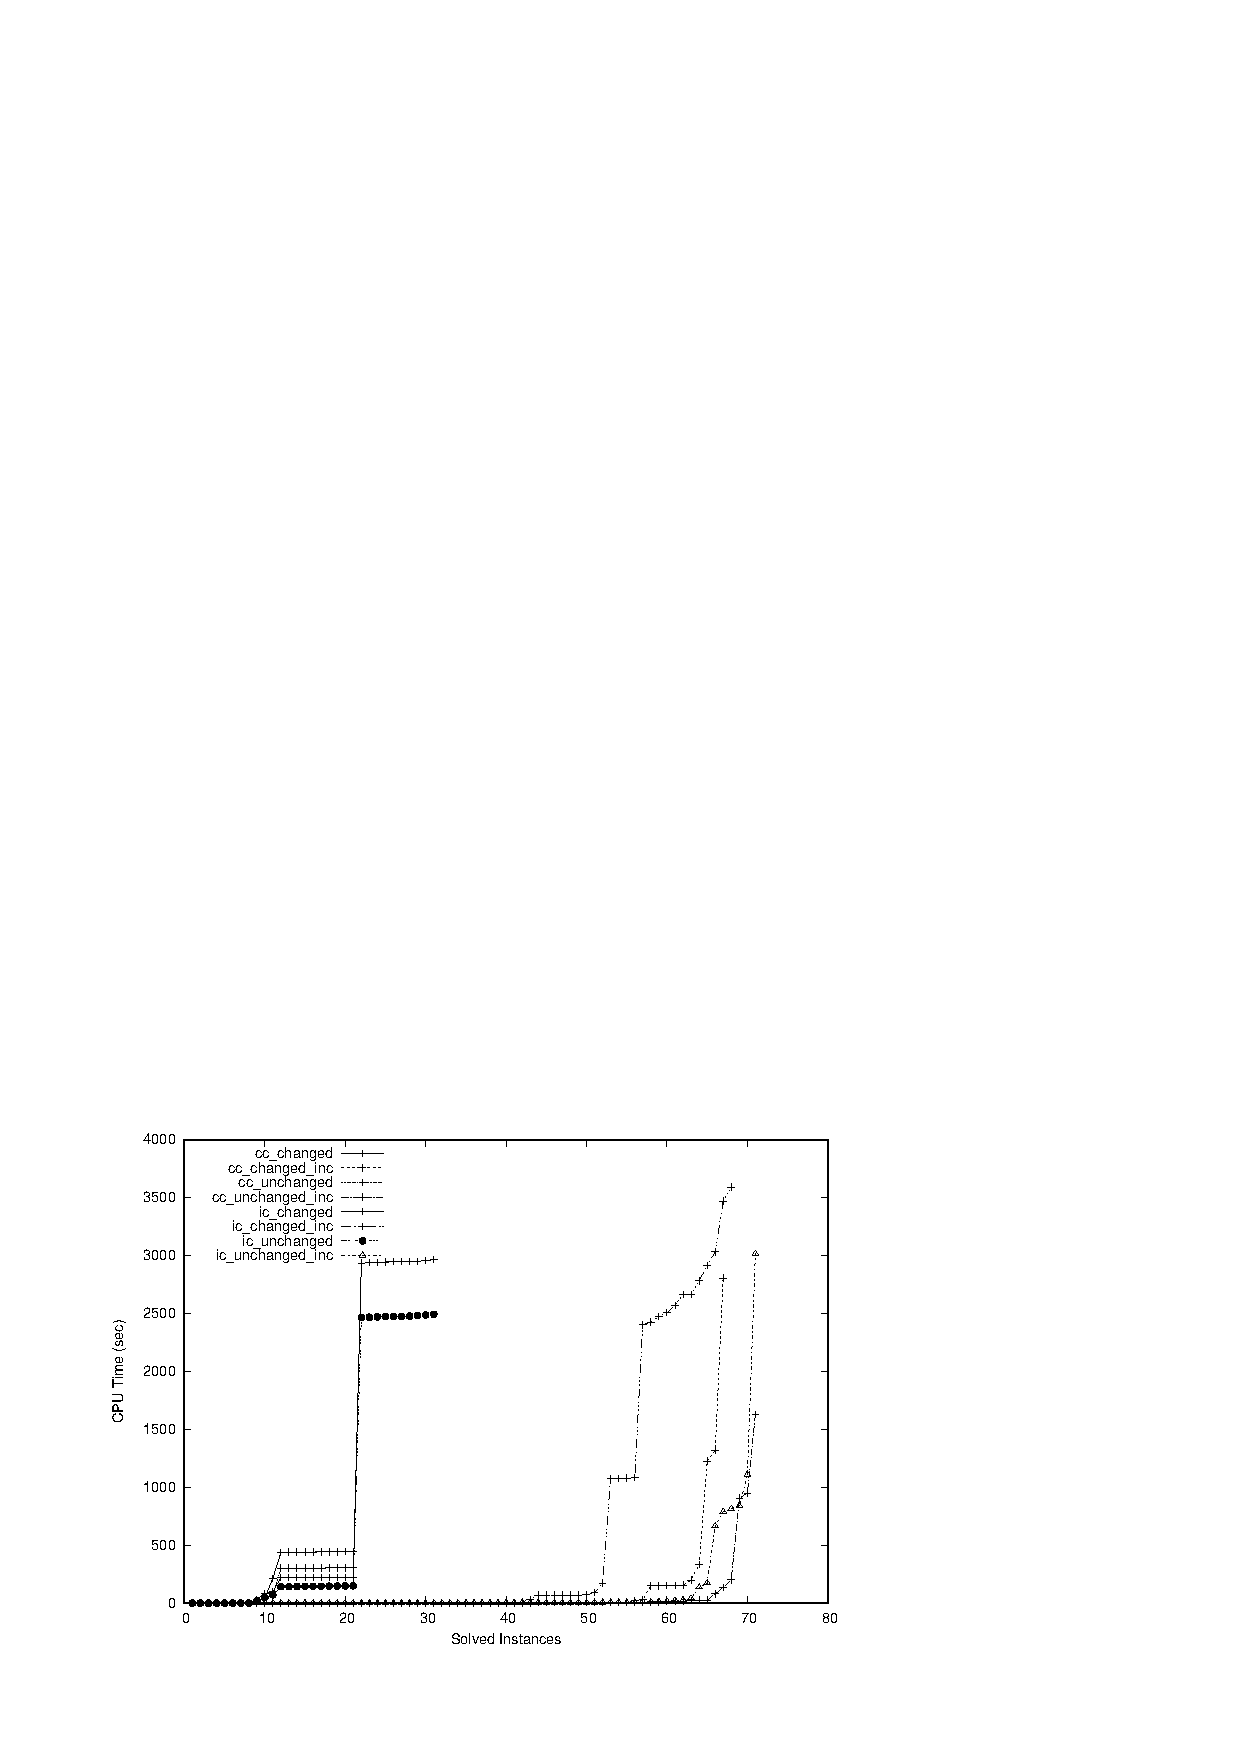
\includegraphics[scale=0.38]{fig/cactus.png}
 \end{figure}

\begin{itemize}
 \item 提案符号化2は,提案符号化1と比較して,より多くの問題を高速に解いている.
\end{itemize}
\end{frame}

%%%%%%%%%%%%%%%%%%%%%%%%%%%%%%%%%%%%%%%%%%%%%%%%%%
%% 辺の数の表
%%%%%%%%%%%%%%%%%%%%%%%%%%%%%%%%%%%%%%%%%%%%%%%%%%
\begin{frame}\frametitle{実験結果(2/2) : 解けた問題数による比較} % 表による比較

\begin{table}[t]
 \centering
 \begin{tabular}[t]{ccccc}
 \rowcolor[RGB]{0,96,0}
 \color{white} 辺の範囲 & \color{white}問題数 & 
		 \color{white}基本符号化 & \color{white}改良符号化 & \color{white}有向符号化\\
 %%%%%%%%
 \rowcolor[RGB]{230,239,230}
 ~~~~\;\:1 ~ 1,000 & 30 & \alert{30} & \alert{30} & \alert{30} \\
 \rowcolor[RGB]{196,230,196}
 1,001 ~ 4,000 & 20 & \alert{20} & \alert{20} & \alert{20} \\
 \rowcolor[RGB]{230,239,230}
 4,001 ~ 7,000 & 11 & 9 & 10 & \alert{11} \\
 \rowcolor[RGB]{196,230,196}
 ~\:7,001 ~ 10,000 & 8 & 4 & 6 &\alert{7} \\
 \rowcolor[RGB]{230,239,230}
 10,001 ~ 20,000 & 9 & 2 & 5 &\alert{9} \\
 \rowcolor[RGB]{196,230,196}
 20,001 ~ 30,000 & 2 & 1 & \alert{2} & \alert{2} \\
 \rowcolor[RGB]{230,239,230}
 30,001 ~ 40,000 & 1 & 0 & 0 & \alert{1} \\
 \rowcolor[RGB]{196,230,196}
 40,001 ~ 50,000 & 4 & 0 & 2 & \alert{4} \\
 %%%%%%%% 合計
 \noalign{\hrule height 0.5pt}
 \rowcolor[RGB]{230,239,230}
 計 & 85 & 66 & 75 & \alert{84} \\
 
\end{tabular}

\end{table}

\begin{itemize}
 \item 大規模な問題に対する提案符号化2の有効性が確認できた.
 \item 提案符号化2は,辺の数が40,000を超える問題も解いた.
\end{itemize}

\end{frame}

%%%%%%%%%%%%%%%%%%%%%%%%%%%%%%%%%%%%%%%%%%%%%%%%%%
%% まとめ
%%%%%%%%%%%%%%%%%%%%%%%%%%%%%%%%%%%%%%%%%%%%%%%%%%
\begin{frame}\frametitle{まとめと今後の課題}
 % 自分が伝えたいことをメインに書く
 \begin{block}{まとめ}
  \begin{enumerate}
   \item \structure{根付き全域森問題を解く,2種類のASP符号化を考案した.}
   \begin{itemize}
	\item ASP言語の表現力を用いて,根付き全域森の制約を簡潔に表現できること
		  が確認できた.(ASPのルールで5つ程度)
   \end{itemize}
   \item \structure{実用規模の問題,及び,より大規模な問題を用いた評価実験.}
   \begin{itemize}
	%	\item 提案符号化2は,提案符号化1よりも多くの問題を高速に解いた.
	\item 提案符号化2は,辺の数が40,000を超えるような問題も解くことが
		  でき,大規模な問題に対する有効性が確認できた.
   \end{itemize}
   \item 遷移問題へ拡張し,その符号化を考案した. (本発表では省略)
  \end{enumerate}
 \end{block}
 
 \begin{alertblock}{今後の課題}
  \begin{itemize}
   \item 電気制約への対応.
		 \begin{itemize}
		  \item ASPMT技術を用いた実装.
		 \end{itemize}
   \item 遷移問題へ拡張した符号化の評価実験.
  \end{itemize}
 \end{alertblock}
\end{frame}

%###########################################################
%##### 補助スライド ########################################
%###########################################################
\begin{frame}{~}
 \centering
 - 補足用 -
\end{frame} 

\begin{frame}{補足 : スマートグリッド}
 \begin{itemize}
  \item \structure{スマートグリッド}とは,電力の供給側,需要側において双方向の
		やり取りを可能にする次世代の\structure{賢い}電力網である.
  \item 従来と違い,通信技術の発達により,使用状況などを
		リアルタイムに把握することが可能となった.
  \item その時に応じた最適な配電網を構成し,制御するといったことが考えられている.
		\begin{itemize}
		 \item 電力需要の変化による,配電ロスの少ない構成.
		 \item 自然エネルギーによる発電量の変動を補う構成.
		\end{itemize}
  \item ASP言語の表現力や拡張性が,こうした条件の追加に活用できる可能性がある.
 \end{itemize}
\end{frame}

%%%%%%%%%%%%%%%%%%%%%%%%%%%%%%%%%%%%%%%%%%%%%%%%%%
%% 電気制約
%%%%%%%%%%%%%%%%%%%%%%%%%%%%%%%%%%%%%%%%%%%%%%%%%%
\begin{frame}{補足 : 電気制約}
 \begin{itemize}
  \item \alert{電気制約}は,送電する電流$\cdot$電圧の適正範囲を保証する制約.
  \begin{itemize}
   \item 供給経路の各区間で許容電流を超えない.
   \item 電気抵抗による電圧降下が許容範囲を超えない.
   \item etc.
  \end{itemize}
  \item 電流と電圧が影響し合う\structure{実数ドメイン上の制約}によって表される.
		% \begin{itemize}
		%  		 \item 送電システム上の条件など.
		% \end{itemize}
  \item 実数ドメイン上の制約は,純粋なASPのみで扱うのは\alert{困難}.
		\begin{itemize}
		 \item 緩和問題として,変電所から供給できる家庭の数に上限をつける.
		 \item ASPMT技術により,ASPで得られた解について,
			   背景理論ソルバーと連携して実数ドメイン上の制約を調べる.
		\end{itemize}
 \end{itemize}
\end{frame}


%%%%%%%%%%%%%%%%%%%%%%%%%%%%%%%%%%%%%%%%%%%%%%%%%%
%% 基礎化
%%%%%%%%%%%%%%%%%%%%%%%%%%%%%%%%%%%%%%%%%%%%%%%%%%
\begin{frame}{補足 : ASPシステム}
 
 \vspace{-0.5cm}

 \begin{figure}[htbp]
  \centering
  %%%%%%%%%%%%%%%%%%%%%%%%%%%%%%%%%%%%%%%%%%%%%%%%%%
%% 基礎化の流れの図
%%%%%%%%%%%%%%%%%%%%%%%%%%%%%%%%%%%%%%%%%%%%%%%%%%
\begin{tikzpicture}

 \definecolor{edge}{RGB}{38,38,134}
 \definecolor{node}{RGB}{220,220,249}

 \definecolor{alert_edge}{RGB}{191,0,0}
 \definecolor{alert_node}{RGB}{249,200,200}

 \definecolor{ex_edge}{RGB}{0,96,0}
 \definecolor{ex_node}{RGB}{230,239,230}

 \def\nodespace{2.4cm}

 \tikzset{block/.style={rectangle, thick, draw=edge, fill=node, text width=3cm, 
 text centered, rounded corners, text width=2cm, minimum height=1.5cm}};

 \tikzset{alertblock/.style={rectangle, thick, draw=alert_edge, fill=alert_node, 
 text width=3cm, text centered, rounded corners, text width=1.5cm, minimum height=1.2cm}};

 \node[block](ikkai){一階ASP\\プログラム};

 \node[rectangle,rounded corners, thick, draw=ex_edge, fill=ex_node, 
 right=0.22*\nodespace of ikkai, minimum width=6cm, minimum height=3cm, 
 text centered, label=ASPシステム](sys){};

 \node[block, right=\nodespace of ikkai](meidai){命題ASP\\プログラム};
 \node[block, right=\nodespace of meidai](ASP){解集合};

 \node[right=0.6*\nodespace of ikkai, text width=1.5cm, 
 text centered, text=red, anchor=south](){基礎化\\ソルバー};
 \node[right=0.4*\nodespace of meidai, text width=1.5cm, 
 text centered, text=red, anchor=south](){解集合\\ソルバー};

 
 \foreach \u / \v / \n in {ikkai/meidai,meidai/ASP}
 \draw [thick,->] (\u) to (\v);

\end{tikzpicture}
 \end{figure}

 \vspace{-0.5cm}

 \begin{exampleblock}{}
  \begin{enumerate}
   \item 一階ASPプログラムを基礎化ソルバーによって,
		 命題ASPプログラムに\alert{基礎化}する.
   \item 命題ASPプログラムについて,SAT技術を応用した解集合ソルバーが解集合を探索する.
  \end{enumerate}
 \end{exampleblock}

\end{frame}

%%%%%%%%%%%%%%%%%%%%%%%%%%%%%%%%%%%%%%%%%%%%%%%%%%
%% 遷移問題
%%%%%%%%%%%%%%%%%%%%%%%%%%%%%%%%%%%%%%%%%%%%%%%%%%
\begin{frame}{補足 : 遷移問題}
 \begin{block}{}
   根付き全域森の制約を満たしたまま,各遷移時に変化できる\\
  辺の数は2つ以下として,遷移を求める.
 \end{block}
 \vspace{-0.15cm}
 \begin{exampleblock}{}
  \begin{figure}[htbp]
   \begin{tabular}[tb]{cc}
	\begin{minipage}{0.5\hsize}
	 \centering
	 \input{tikz/tikz-trans-1}
	 $t=0$ (初期状態)
	\end{minipage}
	& 
	\hspace{-0.5cm}
	\begin{minipage}{0.5\hsize}
	 \centering
	 \input{tikz/tikz-trans-2}
	 $t=1$
	\end{minipage} 
   \end{tabular}\\
   \vspace{0.25cm}
   \begin{tabular}[tb]{cc}
	\begin{minipage}{0.5\hsize}
	 \centering
	 \input{tikz/tikz-trans-3}
	 $t=2$
	\end{minipage}
	&
	\hspace{-0.5cm}
	\begin{minipage}{0.5\hsize}
	\centering
	 %%%%%%%%%%%%%%%%%%%%%%%%%%%%%%%%%%%%%%%%%%%%%%%%%%
% 実行例(t=3) (第6章で使う)
%%%%%%%%%%%%%%%%%%%%%%%%%%%%%%%%%%%%%%%%%%%%%%%%%%
\begin{tikzpicture}[scale=0.6]

 % 設定
 \tikzset{node/.style={circle,draw=black,fill=white}}

 \definecolor{edge1}{RGB}{191,0,0}
 \definecolor{node1}{RGB}{249,200,200}
 \definecolor{edge3}{RGB}{38,38,134}
 \definecolor{node3}{RGB}{200,200,249}

 % 補助線
 % \draw [help lines,blue] (0,0) grid (20,6);

 % node %
 \node[circle, ultra thick, draw=edge1, fill=node1](out1){1};
 \node[node, fill=node3, right=of out1] (out2){2};
 \node[circle, ultra thick, draw=edge3,fill=node3, right=of out2](out3){3};
 \node[node, fill=node3, below=of out1] (out4){4};
 \node[node, fill=node3, below=of out2] (out5){5};
 \node[node, fill=node3, below=of out3] (out6){6};

 \foreach \u / \v in {}
 \draw [very thick, edge1] (\u) -- (\v);

 \foreach \u / \v in {out2/out3,out2/out5,out4/out5,out5/out6}
 \draw [very thick, edge3](\u) -- (\v);
\end{tikzpicture}

%%%%%%%%%%%%%%%%%%%%%%%%%%%%%%%%%%%%%%%%%%%%%%%%%%%%%%%%%%
%%% Local Variables:
%%% mode: japanese-latex
%%% TeX-master: paper.tex
%%% End:

	 $t=3$ (目的状態)
	\end{minipage}
   \end{tabular}
  \end{figure}
 \end{exampleblock}
\end{frame}


%%%%%%%%%%%%%%%%%%%%%%%%%%%%%%%%%%%%%%%%%%%%%%%%%%
%% ASPのコード
%%%%%%%%%%%%%%%%%%%%%%%%%%%%%%%%%%%%%%%%%%%%%%%%%%
\begin{frame}[fragile]{補足 : 提案符号化1のASPプログラム}
 \begin{exampleblock}{}
  \begin{center}
   %%%%%%%%%%%%%%%%%%%%%%%%%%%%%%%%%
   \lstinputlisting[numbers=left,%
   basicstyle=\ttfamily\tiny]{code/srf1.lp}
   %%%%%%%%%%%%%%%%%%%%%%%%%%%%%%%%% 
  \end{center}
 \end{exampleblock}
\end{frame}

\begin{frame}[fragile]{補足 : 提案符号化2のASPプログラム}

 \begin{exampleblock}{}
  \begin{center}
   %%%%%%%%%%%%%%%%%%%%%%%%%%%%%%%%%
   \lstinputlisting[numbers=left,%
   basicstyle=\ttfamily\tiny]{code/srf2.lp}
   %%%%%%%%%%%%%%%%%%%%%%%%%%%%%%%%% 
  \end{center}
 \end{exampleblock}

\end{frame}


\end{document}